\documentclass{standalone}
\usepackage{tikz}
\usepackage{nono}
\begin{document}
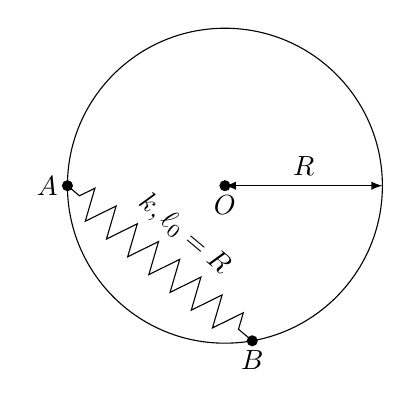
\begin{tikzpicture}
\draw (0,0) circle(2cm);
\fill[black](-2, 0) coordinate (A) circle(2pt) node[left]{$A$};
\fill[black](-80:2) coordinate (B) circle(2pt) node[below]{$B$};
\fill[black](0,0) coordinate (O) circle(2pt) node[below]{$O$};
\draw[decorate,decoration={zigzag,amplitude=0.2cm,pre length=0.2cm,post length=0.2cm}] (A) -- (B) node[midway, above=0.2cm, sloped]{$k, \ell_0=R$} ;
\draw[latex-latex] (O) -- (2,0) node[midway, above]{$R$}; 
\end{tikzpicture}
\end{document}
